\documentclass[a4paper]{article}
\usepackage{graphicx}
%\usepackage{subcaption}
\usepackage[margin=2cm]{geometry}
\usepackage[maxbibnames=9,citestyle=nature,doi=false,isbn=false,url=false,eprint=false]{biblatex}
\usepackage{hyperref}
\hypersetup{
    colorlinks=true,
    linkcolor=blue,
    filecolor=magenta,
    urlcolor=cyan,
}
\usepackage{mathtools}
\usepackage{bm}
\usepackage{caption}
%\usepackage{multirow}
\DeclareCaptionLabelFormat{cont}{#1~#2\alph{ContinuedFloat}}
\captionsetup[ContinuedFloat]{labelformat=cont}
\newcommand{\HRule}{\rule{\linewidth}{0.5mm}}

\title{\textsc{Studying the effects of competition on adaptive therapy}\\\Large{Mid Year Report}}
\author{Harshavardhan BV (20161100), 5th Year BS-MS\\
Under the guidance of Prof. Sutirth Dey, IISER Pune}
\date{January 2021}
\bibliography{References}
\graphicspath{ {./figures/} }

\begin{document}
\maketitle

\section{Introduction}
\subsection{Adaptive therapy}
Conventional therapy against cancer focusses on minimising tumour burden by administering cytotoxic drugs at the maximum tolerated dosage (MTD). However, most tumours are heterogenous in their sensitivity to these drugs, and MTD regimens eliminate the most sensitive cells, allowing the resistant cells to re-establish a resistant population \cite{Scott}. Adaptive therapy aims to reduce such competitive release by administering the drug at a dosage less than the MTD in a fluctuating manner. This allows for some proportion of sensitive cells to survive in the tumour population while reducing the net tumour burden, thus preventing a complete takeover by the resistant phenotype.

\subsection{Metastatic Castration-Resistant Prostate Cancer}
The system of study was chosen to be Metastatic Castration-Resistant Prostate Cancer (mCRPC) since it has a history of adaptive therapy theory work \cite{Cunningham}. mCRPC is composed of three types of cells: $T^+$, $T^p$ and $T^-$. Only $T^+$ and $T^p$ require testosterone for proliferation and survival, and $T^-$ is testosterone-independent. While $T^+$ cannot secrete testosterone, $T^p$ cells produce testosterone through upregulation of the corresponding enzyme, $CYP17\alpha$ and $T^-$ cells have mutations in androgen receptors that allow them to survive without testosterone.

\subsection{Competition between cells}
The success of adaptive therapy in containing the tumour depends on the effectiveness of competition between sensitive and resistant cells. Cells can use different strategies such as higher proliferation rate, better survival at sub-optimal conditions or lower death rate to compete with each other, and several such strategies are seen to be acquired over the course of cancer progression, as shown by the ``hallmarks of cancer" framework \cite{Hanahan}. The role of the choice of strategy on the final outcomes of cell competition and eventually, the efficacy of adaptive therapy, has not yet been studied closely.

\section{Work done till now}
\subsection{ODE Model}
To begin with, a simplistic Ordinary Differential Equation (ODE) model was used. This would help us with forming expectations of the system and parameterization for the upcoming Agent Based Model (ABM). The ODE model is less computationally costly at the tradeoff of not being able to capture complex behaviour when compared to ABM.

We developed a logistic framework modified with a dynamic carrying capacity that depended on environmental conditions. The ``environment" consists of the resources, oxygen and testosterone which have their own equations for production and consumption. We make the simplifying assumption that every other resource required by cells are present in non-limiting concentrations. The equations are given below:
\begin{equation}
  \frac{dy_i}{dt} = r_i y_i (1 - \frac{\sum_j y_j}{1 + K_{i,max} f_i(O_2) f_i(test)} )- \delta_i y_i
  \label{celleq}
\end{equation}
\begin{equation}
  \frac{dO_2}{dt} = p_{O_2} - \sum_i \mu_{O_2,i} y_i - \lambda_{O_2} O_2
  \label{o2eq}
\end{equation}
\begin{equation}
  \frac{dtest}{dt} = p_{test} y_{T^p} - \sum_i \mu_{test,i} y_i - \lambda_{test} test
  \label{testeq}
\end{equation}
\begin{equation}
  f_i(res) = \begin{cases}
    1 &\text{if } ul_{res,i} \leq res\\
    \frac{res-ll_{res,i}}{ul_{res,i}-ll_{res,i}} &\text{if } ll_{res,i} < res < ul_{res,i}\\
    0 &\text{if } res \leq ll_{res,i}\\
  \end{cases}
  \label{freseq}
\end{equation}

$i \in \{T^+,T^p,T^-\}$ and $res \in \{O_2,test\}$.

\subsection{Parameters and Standardization}
A major portion of the time was spent in standardising the model with suitable parameters. Table \ref{parmtable} gives a brief description of the parameters from the above equations, the values used, and the sources for these values where applicable. Note that all the resource parameters are normalised to tissue levels of that resource.\\
Constraint equations given below were used to determine the values of some parameters for which direct sources were not available.
\begin{equation}
  r_i = \frac{ln(2)}{\tau_{d,i}} + \delta_i
  \label{r_eq}
\end{equation}
\begin{equation}
  K_{i,max}=\frac{r_i}{r_i-\delta_i} y_i^*
  \label{rho_eq}
\end{equation}
\begin{equation}
  p_{O_2} = \lambda_{O_2} O_2^* + y_i^* \mu_i
  \label{p_o2_eq}
\end{equation}
\begin{equation}
  p_{test} - \mu_{test,T^p} = \frac{test^* \lambda_{test}}{y_{T^p}^*} = 4 \times 10^{-4}
  \label{p_test_eq}
\end{equation}
\begin{table}[t]
  \centering
  \begin{tabular}{|l|p{5cm}|c|l|}
    \hline
    \textbf{Parameter}  & \textbf{Description} & \textbf{Value(s)} & \textbf{Source(s)} \\ \hline
    $y_i$ & No. of cells of cell type $i$ & N/A & N/A  \\ \hline
    $r_i$ & Population growth rate of cell type i  &
    \begin{tabular}{l|l}
      $T^+$ & $2.84 \times 10^{-3}$ min$^{-1}$\\
      $T^p$ & $2.79 \times 10^{-3}$ min$^{-1}$\\
      $T^-$ & $6.23 \times 10^{-4}$ min$^{-1}$\\
    \end{tabular}
    & Eq \ref{r_eq} \\ \hline
    $\delta_i$  & Population death rate of cell type i &
    \begin{tabular}{l|l}
      $T^+$ & $2.5 \times 10^{-3}$ min$^{-1}$\\
      $T^p$ & $2.5 \times 10^{-3}$ min$^{-1}$\\
      $T^-$ & $1.6 \times 10^{-4}$ min$^{-1}$\\
    \end{tabular}
    & \cite{Jain}  \\ \hline
    $K_{i,max}$ & Maximum Carrying capacity, coming up through the environment/resources &
    \begin{tabular}{l|l}
      $T^+$ & $8.35 \times 10^4$ \\
      $T^p$ & $9.62 \times 10^4$ \\
      $T^-$ & $1.34 \times 10^4$ \\
    \end{tabular}
    & Eq \ref{rho_eq} \\ \hline
    $f_{i,res}$ & Functional dependence of cell type $i$ on resource $res$, normalised to 1 & $f_{T^-,test}=1$ & N/A \\ \hline
    $p_{res}$ & Production rate of resource, either as bulk or by cells &
    \begin{tabular}{l|l}
      $O_2$ & 0.11 min$^{-1}$\\
      $test$ & $5 \times 10^{-7}$ min$^{-1}$cell$^{-1}$\\
    \end{tabular}
    & Eqs \ref{p_o2_eq},\ref{p_test_eq}\\ \hline
    $\mu_{res,i}$ & Uptake of resource $res$ by cell type $i$ &
    \begin{tabular}{l|l|l}
      $O_2$ & $T^+$ & $1.63 \times 10^{-6}$ min$^{-1}$cell$^{-1}$\\
      & $T^p$ & $1.63 \times 10^{-6}$ min$^{-1}$cell$^{-1}$\\
      & $T^-$ & $1.04 \times 10^{-6}$ min$^{-1}$cell$^{-1}$\\ \hline
      $test$ & $T^+$ & $2.34 \times 10^{-8}$ min$^{-1}$cell$^{-1}$\\
      & $T^p$ & $6.00 \times 10^{-8}$ min$^{-1}$cell$^{-1}$\\
      & $T^-$ & 0 min$^{-1}$cell$^{-1}$\\
    \end{tabular}
    & \cite{HailJr}, Eq \ref{p_test_eq}\\ \hline
    $\lambda_{res}$ & Decay rate of resource $res$ &
    \begin{tabular}{l|l}
      $O_2$ & 0.100 min$^{-1}$\\
      $test$ & 0.004 min$^{-1}$\\
    \end{tabular}
    & \cite{Jain}\\ \hline
    $ll_{res,i}$ & Lower limit/threshold level of resource $res$ for carrying capacity of cell type $i$ & $\in [0,1]$ & N/A \\ \hline
    $ul_{res,i}$ & Upper limit/saturation level of resource $res$ for carrying capacity of cell type $i$ & $\in [0,1]$ & N/A \\ \hline
    \multicolumn{4}{|c|}{Supplementary Parameters}\\ \hline
    $\tau_d$  & Doubling time of cell type $i$ &
    \begin{tabular}{l|l}
      $T^+$ & $34$ hr \\
      $T^p$ & $40$ hr \\
      $T^-$ & $25$ hr \\
    \end{tabular}
    & \cite{atcc} \\ \hline
    $y_i^*$ & Equilibrium value of cell number in absence of competition & 10000 & assumed \\ \hline
    $res^*$ & Equilibrium/Tissue levels of resource with one cell type present &
    \begin{tabular}{l|l}
      $O_2$    & 2.5 mmHg          \\
      $test$   & 3.74 pmol/g tissue\\
    \end{tabular}
    & \cite{Steward},\cite{Titus} \\ \hline

  \end{tabular}
  \caption{Table of all parameters}
  \label{parmtable}
\end{table}

\subsection{Pairwise Competition}
With the standardized model, runs with $T^p - T^-$, and $T^+ - T^p$ were done over some combinations of parameters. From the runs, the following observations were made:
\begin{itemize}
  \item In the $T^p - T^-$ pair:
  \begin{enumerate}
    \item $T^p$ is limited by both testosterone and oxygen, whereas $T^-$ is only limited by oxygen. The testosterone limitation is controlled through the two thresholds, $ll_{test,T^p}$ and $ul_{test,T^p}$ as shown in equation \ref{freseq}.
    \item Only when $ul_{test,T^p}$ is low signifying that $T^p$ is not severely testosterone limited, $T^p$ can coexist with or outcompete $T^-$ as shown in Figure \ref{fig_Tpro-Tneg}. In every other case, $T^-$ drives $T^p$ to extinction.
    \item  When $ll_{O2,T-}$ is large , $T^-$ is strongly oxygen-limited but $T^p$ is also limited by testosterone. In this case, $T^-$ wins out eventually as oxygen levels rise faster than testosterone through the external supply term, $p_{O_2}$.
    \item These competitive outcomes are also dependent on the initial proportion of $T^p$, all the other parameters being the same as shown in Figure \ref{fig_Tpro-Tneg}.
  \end{enumerate}
  \item In the $T^+ - T^p$ pair:
  \begin{enumerate}
    \item Both $T^+$ and $T^p$ are limited by both oxygen and testosterone, and compete for both resources. As with the other pair, strength of limitation for any particular resource can be modulated through the corresponding upper and lower thresholds.
    \item When both are severly limited by testosterone, $T^+$ can consume and grow on the limited testosterone present, and this is enough for the density-dependent competition to drive $T^p$ to extinction. Without $T^p$ to provide testosterone, $T^+$ subsequently goes extinct.
    \item When only $T^+$ is severly limited by oxygen and $T^p$ is not, $T^p$ is able to utilise the initial period to grow and secrete enough testosterone to sustain a small $T^+$ population provided the latter do not extinct before then as shown in Figure \ref{fig_Tpos-Tpro_o2lims}.
    \item When $T^p$ is weakly limited by testosterone relative to $T^+$ ($ul_{test,Tp} \leq ul_{test,T+}$), both cells coexist. Due to weaker testosterone limitation, $T^p$ can grow faster initially and secrete enough testosterone for $T^+$ without being negatively affected by $T^+$ as shown in Figure \ref{fig_Tpos-Tpro_testlims}.
    \item In the above case, the proportion of $T^+$ in the final population decreases as $T^+$ becomes more testosterone limited.
  \end{enumerate}
\end{itemize}
\begin{figure}[h]
  \centering
  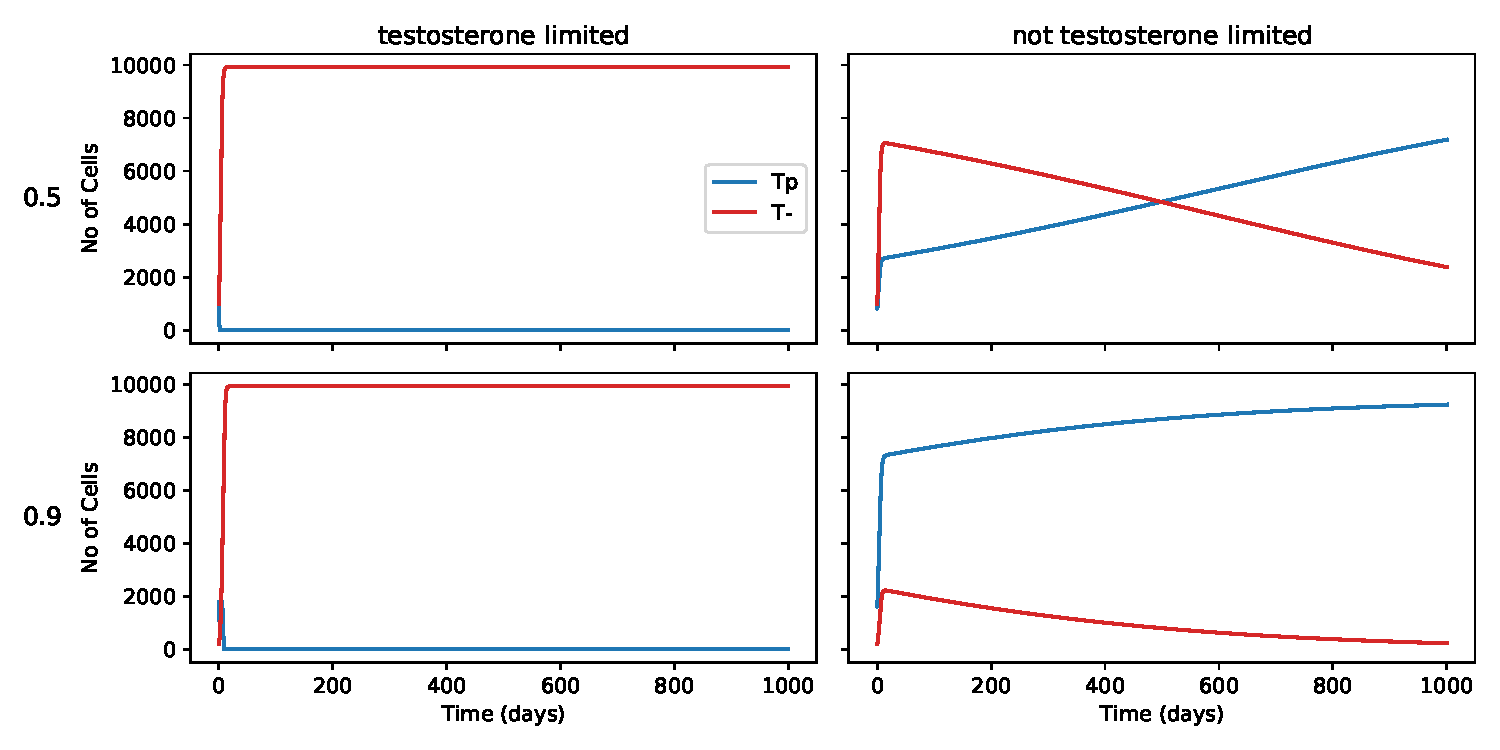
\includegraphics[width=\textwidth]{Tpro-Tneg}
  \caption{Pairwise $T^p - T^-$ timeseries, when $T^p$ is testosterone limited and not testosterone limited (colums) and at different initial proportions of $T^p$(rows). $T^p$ is testosterone limited at $ul_{test,T^p}=0.5$ and not testosterone limited at $ul_{test,T^p}=0.1$.}
  \label{fig_Tpro-Tneg}
\end{figure}
\begin{figure}[h!]
  \centering
  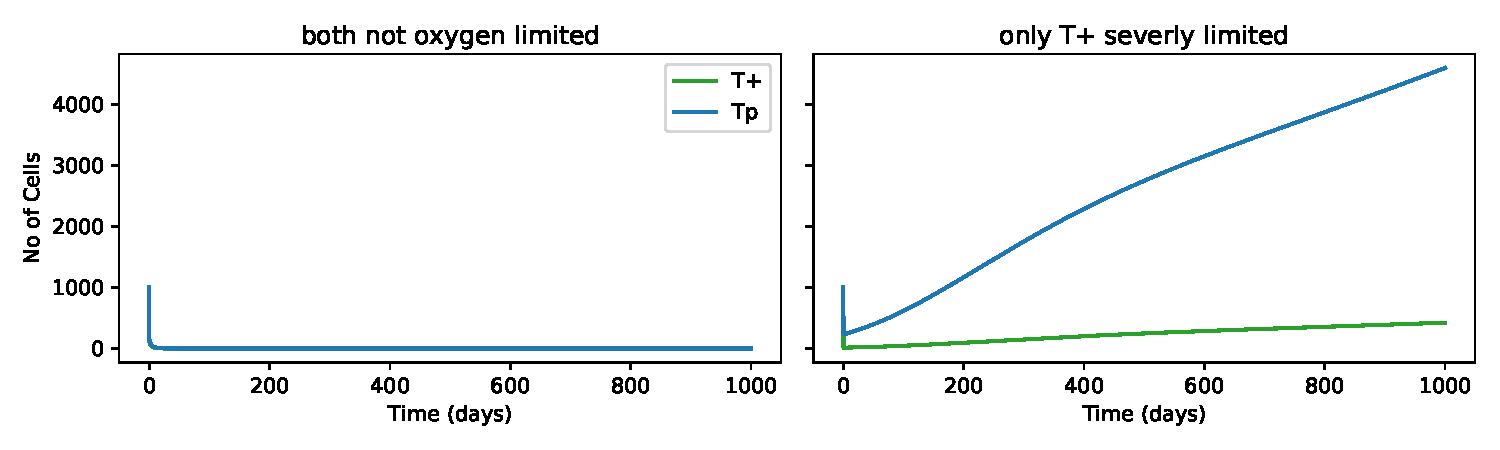
\includegraphics[width=\textwidth]{Tpos-Tpro_o2lims}
  \caption{Pairwise $T^+ - T^p$ timeseries, when both cell types are testosterone limited and not oxygen limited and when $T^+$ is limited more than $T^p$. Both are not oxygen limited at $ul_{O_2,T^+}=0.4,ul_{O_2,T^p}=0.4$ and $T^+$ is severly oxygen limited at $ul_{O_2,T^+}=0.6,ul_{O_2,T^p}=0.4$.}
  \label{fig_Tpos-Tpro_o2lims}
\end{figure}
\begin{figure}[h!]
  \centering
  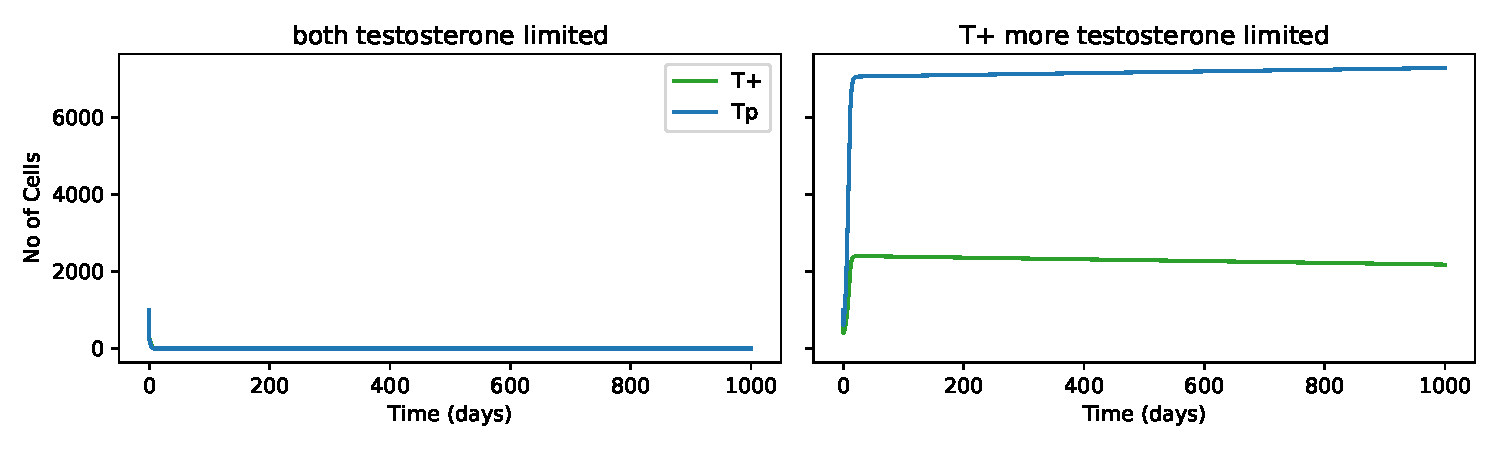
\includegraphics[width=\textwidth]{Tpos-Tpro_testlims}
  \caption{Pairwise $T^+ - T^p$ timeseries, when both cell types are testosterone limited and when $T^+$ is limited more than $T^p$. Both are testosterone limited at $ul_{test,T^+}=0.7,ul_{test,T^p}=0.9$ and $T^+$ is limited more at $ul_{test,T^+}=0.5,ul_{test,T^p}=0.3$.}
  \label{fig_Tpos-Tpro_testlims}
\end{figure}

\section{Future Plans}
From these observations, it is clear that strength of resource limitation affects competitive outcomes. More runs have to be done where the testosterone limitation is relaxed. The oxygen limit needs exploration with lower $ul_{test,i}$ than currently done. Alternatively, oxygen can be made more limiting than testosterone by changing the production rates of these resources.

After this, we plan to move onto competitive runs between all three cell types and then towards simulating different regimens of adaptive therapy. Therapy in this model would involve a $p_{test} = f(dose)$.

Parallely an ABM would be developed which has spatially explicity positioning of cells and diffusion of resources. The simulations run with ODE model would be replicated in the ABM and a comparison between the outcomes would be made.

\printbibliography
\end{document}
